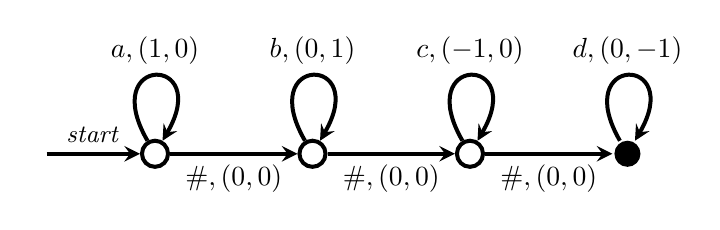
\begin{tikzpicture}
    \node (s) at (-1.5, 0) {};
    \node[draw, circle, minimum size = 0.1in, line width = 0.02in] (a) at (0,0) {};
    \node[draw, circle, minimum size = 0.1in, line width = 0.02in] (b) at (2,0) {};
    \node[draw, circle, minimum size = 0.1in, line width = 0.02in] (c) at (4,0) {};
    \node[fill, circle, minimum size = 0.1in, line width = 0.02in] (d) at (6,0) {};
    
    \draw[-stealth, line width = 0.02in] (s) -- node[above] {\small\textit{start}} (a);
    \draw[-stealth, line width = 0.02in] (a) -- node[below] {$\#, (0, 0)$} (b);
    \draw[-stealth, line width = 0.02in] (b) -- node[below] {$\#, (0, 0)$} (c);
    \draw[-stealth, line width = 0.02in] (c) -- node[below] {$\#, (0, 0)$} (d);
    
    \draw[-stealth, line width = 0.02in] (a) edge[loop above, distance = 0.5in, out=120, in=60] node[above] {$a, (1, 0)$} (a);
    \draw[-stealth, line width = 0.02in] (b) edge[loop above, distance = 0.5in, out=120, in=60] node[above] {$b, (0, 1)$} (b);
    \draw[-stealth, line width = 0.02in] (c) edge[loop above, distance = 0.5in, out=120, in=60] node[above] {$c, (-1, 0)$} (c);
    \draw[-stealth, line width = 0.02in] (d) edge[loop above, distance = 0.5in, out=120, in=60] node[above] {$d, (0, -1)$} (d);
\end{tikzpicture}